\section{Caracterización de datos de trayectorias individuales}
\label{sec:caracterizacion}
El análisis de datos comienza con una etapa fundamental: la caracterización del conjunto de datos. Esta fase tiene como objetivo examinar y comprender la estructura, el contenido y las principales propiedades de los datos antes de aplicar técnicas analíticas más complejas. 
En el caso de los datos de trayectorias individuales, la caracterización permite identificar posibles inconsistencias, redundancias y elementos irrelevantes que puedan afectar la calidad del análisis. Las tareas principales llevadas a cabo en esta etapa son las siguientes:
\begin{itemize}
    \item Explorar las primeras filas del conjunto de datos para obtener una visión general de su estructura.
    \item Verificar la cantidad total de registros y columnas disponibles.
    \item Identificar y eliminar columnas que no aportan información relevante para el análisis o inconsistentes.
    \item Identificar y eliminar las filas que no aportan información relevante para el análisis o inconsistentes.
\end{itemize}
A continuación, se describen en detalle las acciones específicas realizadas durante el proceso de caracterización.
\vfill

% --------------------------
% EXPLORACIÓN INCIAL DEL CONJUNTO DE DATOS
% --------------------------
\subsection{Exploración inicial del conjunto de datos}
\label{subsec:exploracion_inicial}
Como primer paso en la caracterización, se realizó una exploración preliminar del conjunto de datos con el fin de comprender su estructura general. Para ello, se inspeccionaron las primeras dos filas, lo cual permitió identificar las columnas presentes y observar ejemplos representativos de sus valores.
El código utilizado para realizar esta exploración se encuentra en el Apéndice \ref{cod:csv_glance}. A continuación, se presenta un resumen de las columnas detectadas junto con una muestra de sus respectivos valores:

\begin{enumerate}[leftmargin=*, align=left, noitemsep]
    \item \texttt{id}: Identificador numérico único por registro \\
    \footnotesize{\texttt{['34284565','34284566']}}
    \normalsize
    
    \item \texttt{identifier}: UUID del dispositivo \\ 
    \footnotesize{\texttt{['f2640430-7e39-41b7-80bb-3fddaa44779c']}}
    \normalsize

    \item \texttt{identifier\_type}: Tipo de ID (ej. \texttt{'gaid'} para Android) \\ 
    \footnotesize{\texttt{['gaid', 'gaid']}}
    \normalsize

    \item \texttt{timestamp}: Fecha-hora del registro \\ 
    \footnotesize{\texttt{['2022-11-07 02:04:21']}}
    \normalsize

    \item \texttt{device\_lat}/\texttt{device\_lon}: Coordenadas GPS \\ 
    \footnotesize{\texttt{['21.843149']}, \texttt{['-102.196838']}}
    \normalsize

    \item \texttt{country\_short}/\texttt{province\_short}: Códigos de ubicación \\ 
    \footnotesize{\texttt{['MX']}, \texttt{['MX.01']}}
    \normalsize

    \item \texttt{ip\_address}: Dirección IPv6 \\ 
    \footnotesize{\texttt{['2806:103e:16::']}}
    \normalsize

    \item \texttt{device\_horizontal\_accuracy}: Precisión GPS en metros \\ 
    \footnotesize{\texttt{['8.0']}}
    \normalsize

    \item \texttt{source\_id}: Hash de la fuente de datos \\ 
    \footnotesize{\texttt{['449d086d...344']}}
    \normalsize

    \item \texttt{record\_id}: Hash único por registro \\ 
    \footnotesize{\texttt{['77d795df...']}}
    \normalsize

    \item \texttt{home\_country\_code}: País de residencia \\ 
    \footnotesize{\texttt{['MX']}}
    \normalsize

    \item \texttt{home\_geog\_point}/\texttt{work\_geog\_point}: Coordenadas en WKT \\ 
    \footnotesize{\texttt{['POINT(-102.37038 22.20753)']}}
    \normalsize

    \item \texttt{home\_hex\_id}/\texttt{work\_hex\_id}: ID hexagonal (H3) \\ 
    \footnotesize{\texttt{['85498853fffffff']}}
    \normalsize

    \item \texttt{data\_execute}: Fecha de procesamiento \\ 
    \footnotesize{\texttt{['2023-05-30']}}
    \normalsize

    \item \texttt{time\_zone\_name}: Zona horaria \\ 
    \footnotesize{\texttt{['America/Mexico\_City']}}
    \normalsize
\end{enumerate}
\vfill

% --------------------------
% DIMENSIONES DEL CONJUNTO DE DATOS
% --------------------------
\subsection{Dimensiones del conjunto de datos}
\label{subsec:dimensiones}
Para verificar las dimensiones del conjunto de datos, se utilizó la bilbioteca Dask, que permite trabajar con grandes volúmenes de datos de manera eficiente. Junto con Python se usó el código en el Apéndice \ref{cod:csv_count}. Como resultado ahora sabemos que el conjunto de datos contiene un total de \textbf{69,980,000} registros y \textbf{19} campos. Esto indica que hay una cantidad significativa de datos disponibles para el análisis.

% --------------------------
% DEPURACIÓN DE COLUMNAS
% --------------------------
\subsection{Depuración de columnas}
\label{subsec:depuracion_columnas}
Dado que el conjunto de datos original contiene 19 campos, es fundamental identificar y eliminar aquellas columnas que no aportan valor al análisis. Para ello, se realizó una revisión de los valores únicos presentes en cada campo, con el objetivo de detectar información redundante o irrelevante. A partir de este análisis, se identificaron las siguientes columnas como innecesarias para los fines del estudio:

\begin{itemize}
    \item \texttt{id}
    \item \texttt{identifier\_type}
    \item \texttt{country\_short}
    \item \texttt{province\_short}
    \item \texttt{ip\_address}
    \item \texttt{source\_id}
    \item \texttt{home\_country\_code}
    \item \texttt{home\_geog\_point}
    \item \texttt{work\_geog\_point}
    \item \texttt{home\_hex\_id}
    \item \texttt{work\_hex\_id}
    \item \texttt{data\_execute}
\end{itemize}

En lugar de eliminar columnas explícitamente, se optó por seleccionar únicamente aquellas que se desean conservar. El código utilizado para esta tarea se encuentra incluido en el Apéndice \ref{cod:csv_slim}. Dicho script emplea la biblioteca \texttt{dask} para cargar y guardar una nueva versión del conjunto de datos que contiene exclusivamente las siguientes columnas relevantes:

\begin{itemize}
    \item \texttt{identifier}
    \item \texttt{timestamp}
    \item \texttt{device\_lat}
    \item \texttt{device\_lon}
    \item \texttt{device\_horizontal\_accuracy}
    \item \texttt{record\_id}
    \item \texttt{time\_zone\_name}
\end{itemize}

Como resultado, se genera un nuevo archivo \texttt{CSV} que conserva únicamente la información útil para el análisis posterior, optimizando así el tamaño y la calidad del conjunto de datos.


% --------------------------
% DEPURACIÓN DE FILAS
% --------------------------
\subsection{Depuración de filas}
\label{subsec:depuracion_filas}

Una vez obtenida una versión más ligera del conjunto de datos, el siguiente paso consiste en identificar y eliminar aquellas filas que no aportan valor al análisis. Para ello, se generaron representaciones gráficas que permiten observar la distribución de los datos y facilitar la toma de decisiones. Las columnas seleccionadas para este proceso fueron:

\begin{itemize}
    \item \texttt{identifier}: Identificador único del dispositivo.
    \item \texttt{device\_horizontal\_accuracy}: Precisión del GPS en metros. A menor valor, mayor precisión.
\end{itemize}

La primera columna a analizar será \texttt{device\_horizontal\_accuracy}, que refleja la precisión del GPS en metros. Este valor depende tanto del sistema de medición como de la fuente de datos, y suele clasificarse según la siguiente escala:

\begin{itemize}
    \item GPS puro (satelital): 1–20 metros.
    \item A-GPS (asistido por red): 5–50 metros.
    \item Triangulación por WiFi o redes móviles: 20–500 metros.
    \item Geolocalización por IP: 1000–5000 metros.
\end{itemize}

Con base en esta escala,  primero hay que identificar el rango de valores presentes en la columna. Para ello se utilizó el código mostrado en el Apéndice \ref{cod:unique_values}, el cual extrae los valores únicos de \texttt{device\_horizontal\_accuracy} y los guarda en un archivo de texto. El resultado indicó que los valores oscilan entre 0.916 y 199.9, lo que permitió construir un histograma (Apéndice \ref{cod:accuracy_histogram}) para analizar la frecuencia de cada valor y así evaluar su relevancia para el análisis.

El resultado se muestra en la siguiente figura:

\begin{figure}[H]
    \centering
    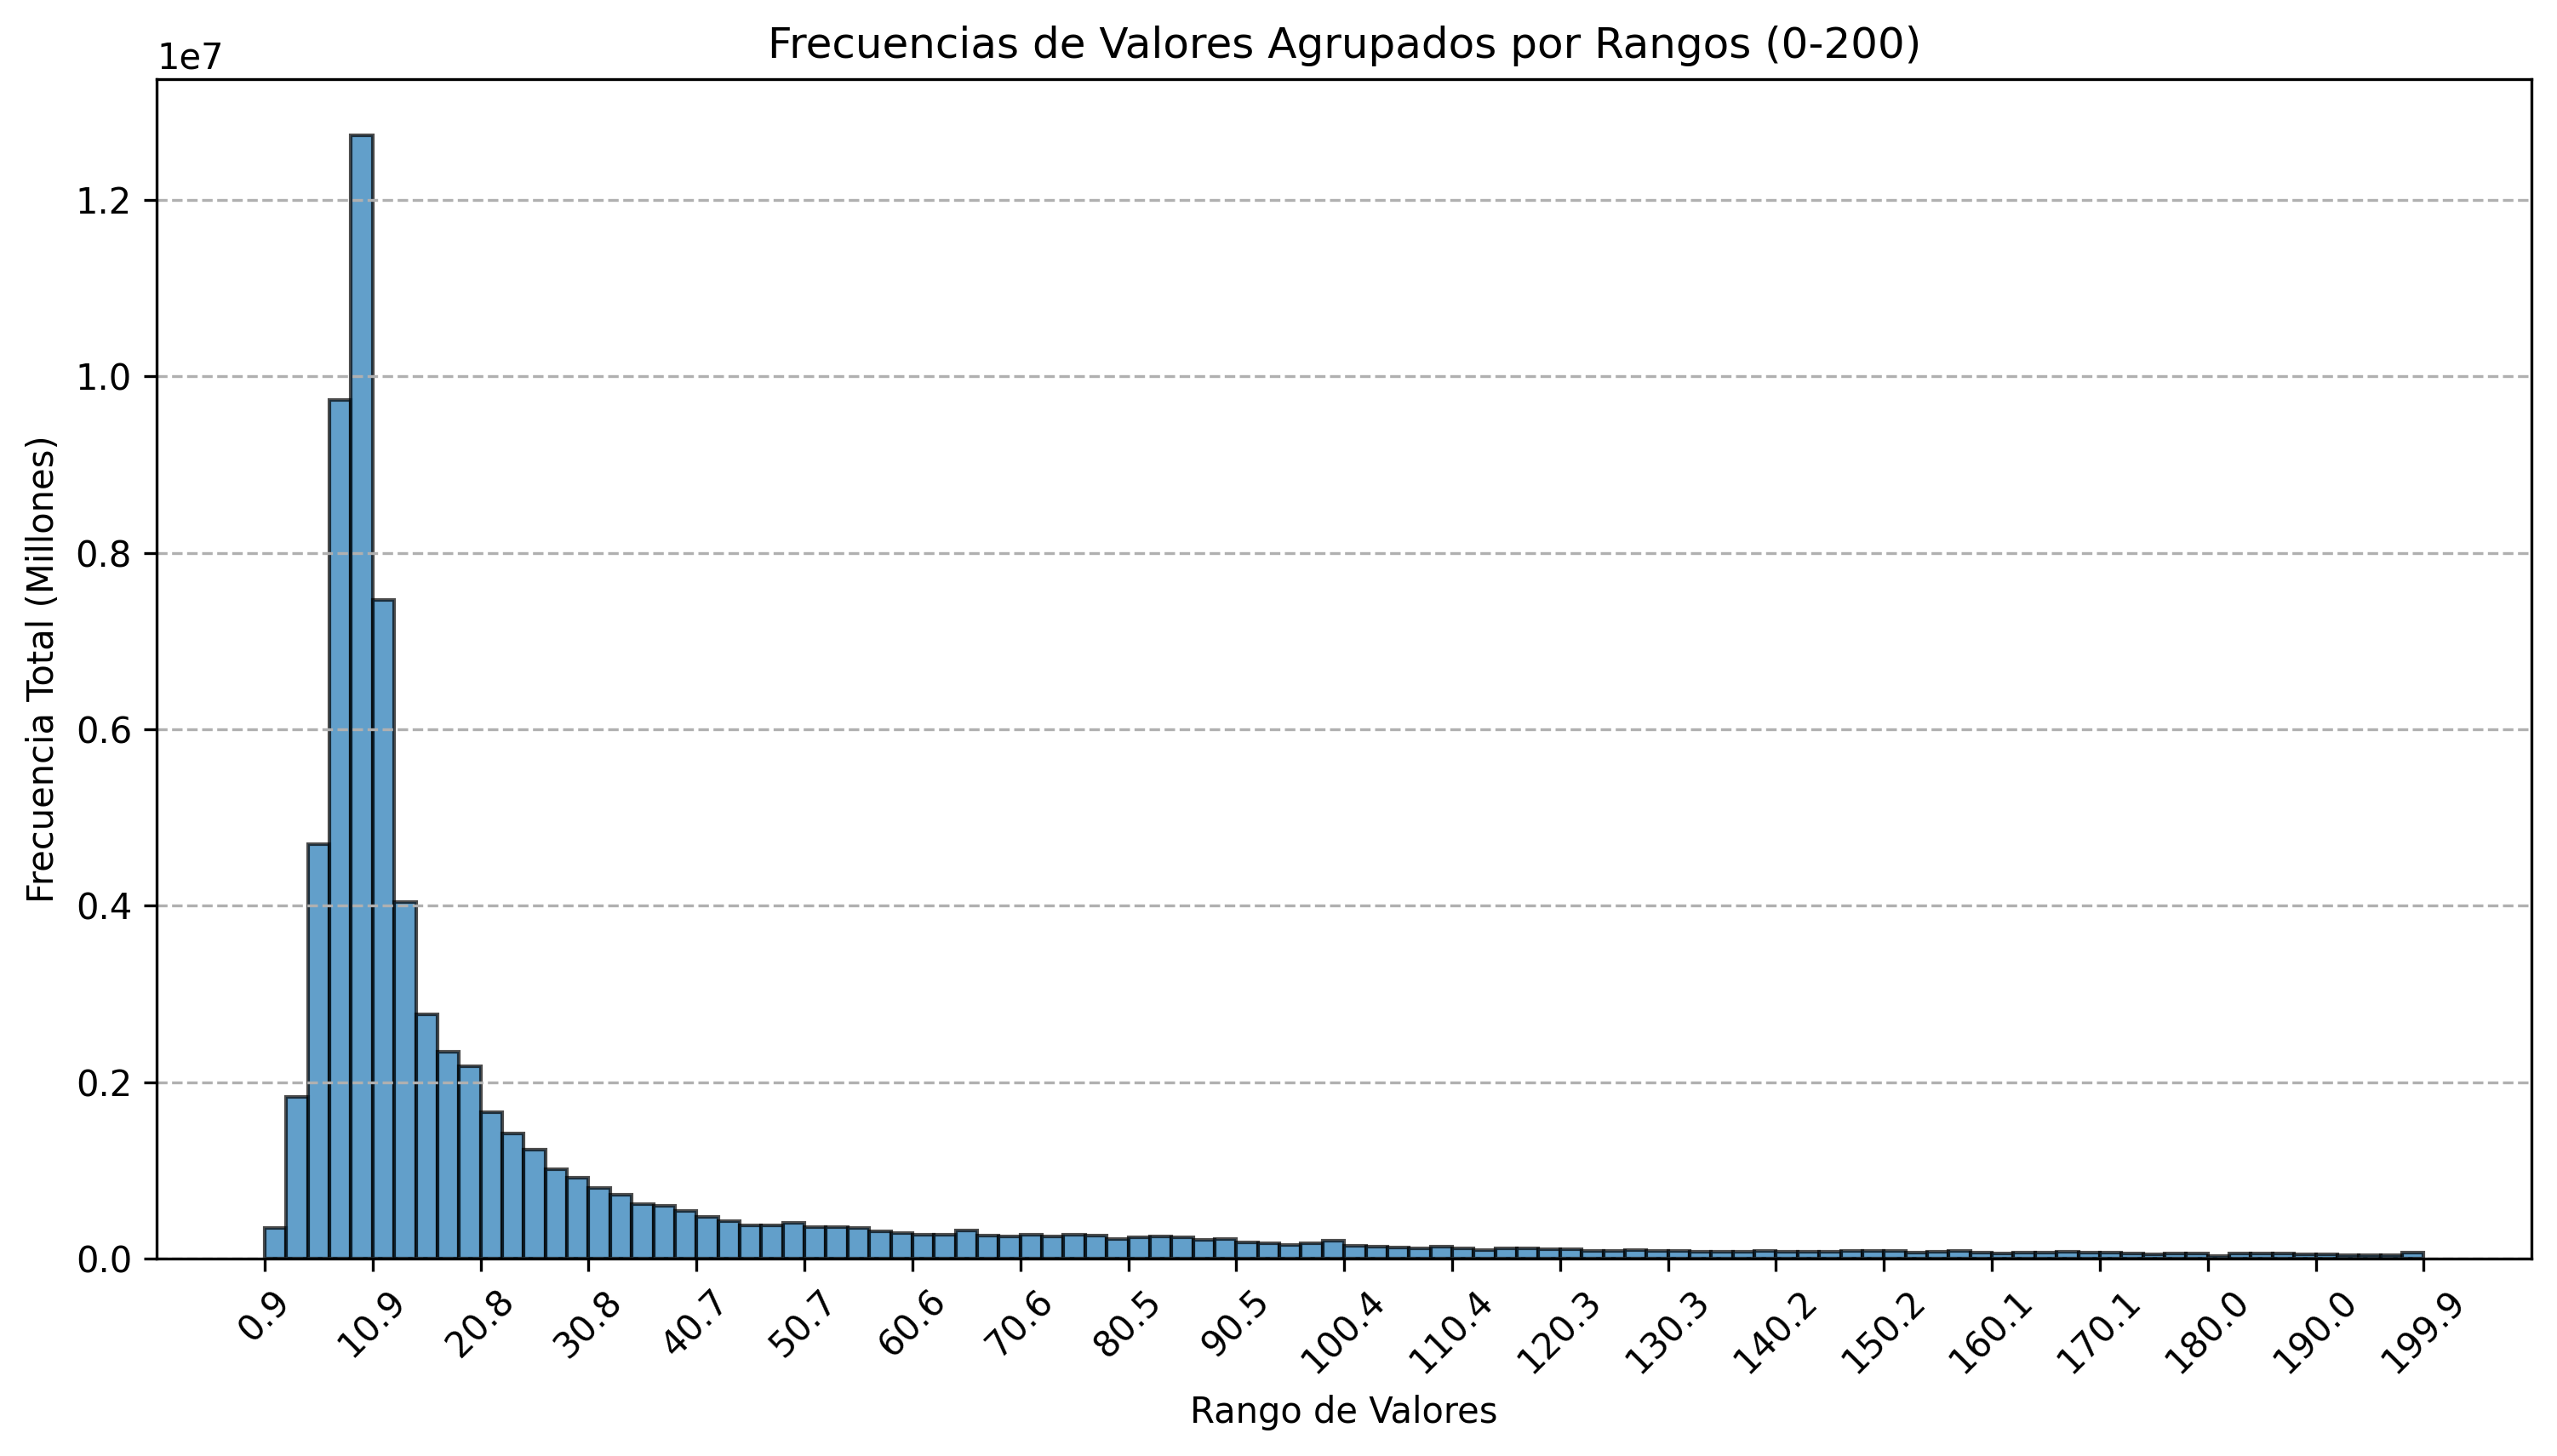
\includegraphics[width=\textwidth]{img/histograma_frecuencias_accuracy.png}
    \caption{Frecuencias de valores agrupados por rangos (0–200 metros).}
    \label{fig:accuracy_histogram}
\end{figure}

Como se observa en la Figura \ref{fig:accuracy_histogram}, la mayoría de los valores se concentran en el rango de 0 a 20 metros, lo cual es consistente con la precisión obtenida mediante GPS puro. Para reforzar esta observación, se realizó un conteo porcentual por tipo de tecnología de geolocalización:

\begin{itemize}
    \item GPS puro (1–20 metros): 68.73\%.
    \item A-GPS (5–50 metros): 16.56\%.
    \item WiFi/red móvil (20–500 metros): 14.69\%.
\end{itemize}

\newpage

La siguiente columna evaluada fue \texttt{identifier}, correspondiente al identificador único de cada dispositivo. Se analiza la frecuencia de aparición de estos valores, para lo cual se empleó un script que agrupa las repeticiones por rangos y grafica la cantidad de valores únicos usando escala logarítmica (ver Apéndice \ref{cod:identifier_histogram}).

\begin{figure}[H]
    \centering
    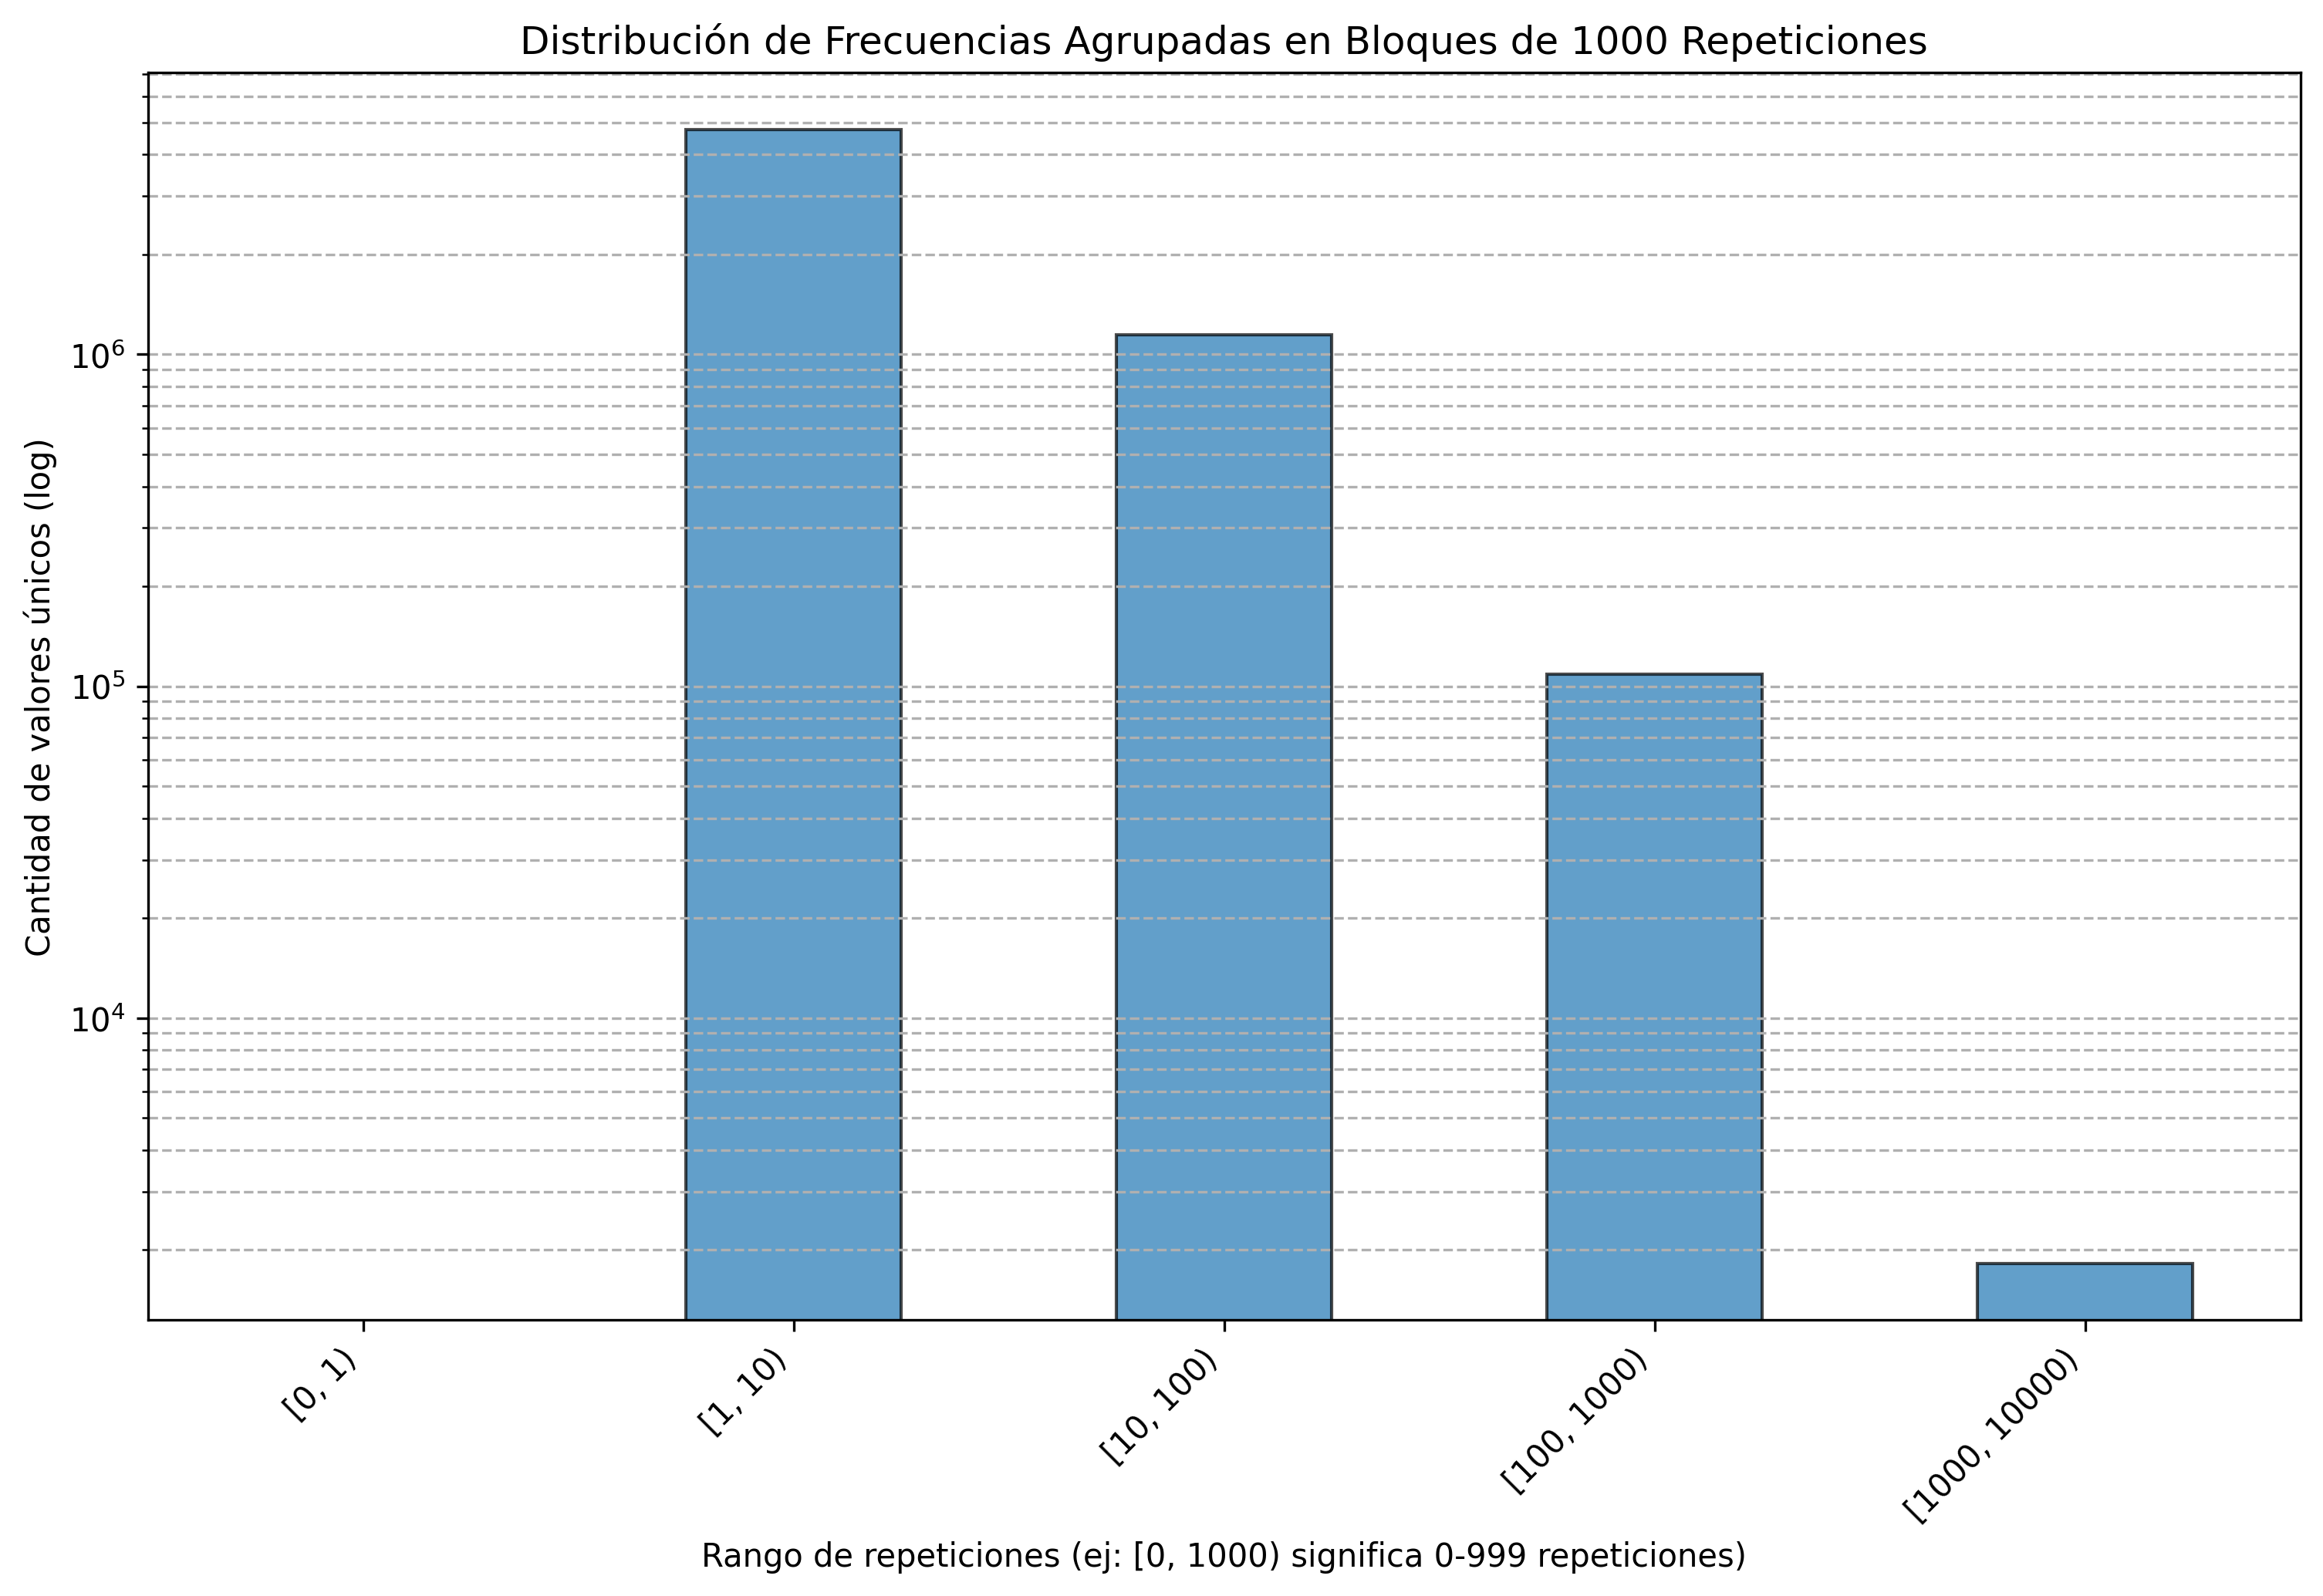
\includegraphics[scale=0.5]{img/histograma_frecuencias_agrupadas_1000.png}
    \caption{Distribución de frecuencias agrupadas en bloques de 1000 repeticiones.}
    \label{fig:identifier_histogram}
\end{figure}

La Figura \ref{fig:identifier_histogram} muestra que la mayoría de los identificadores tienen una baja frecuencia. Para un análisis más detallado, se usó el código del Apéndice \ref{cod:identifier_histogram_detailed}, el cual segmenta los datos en tres rangos: 1–100, 100–1000 y 1000–10000 repeticiones.

\begin{figure}[htbp]
    \centering
    \begin{subfigure}[t]{0.48\textwidth-1em}
        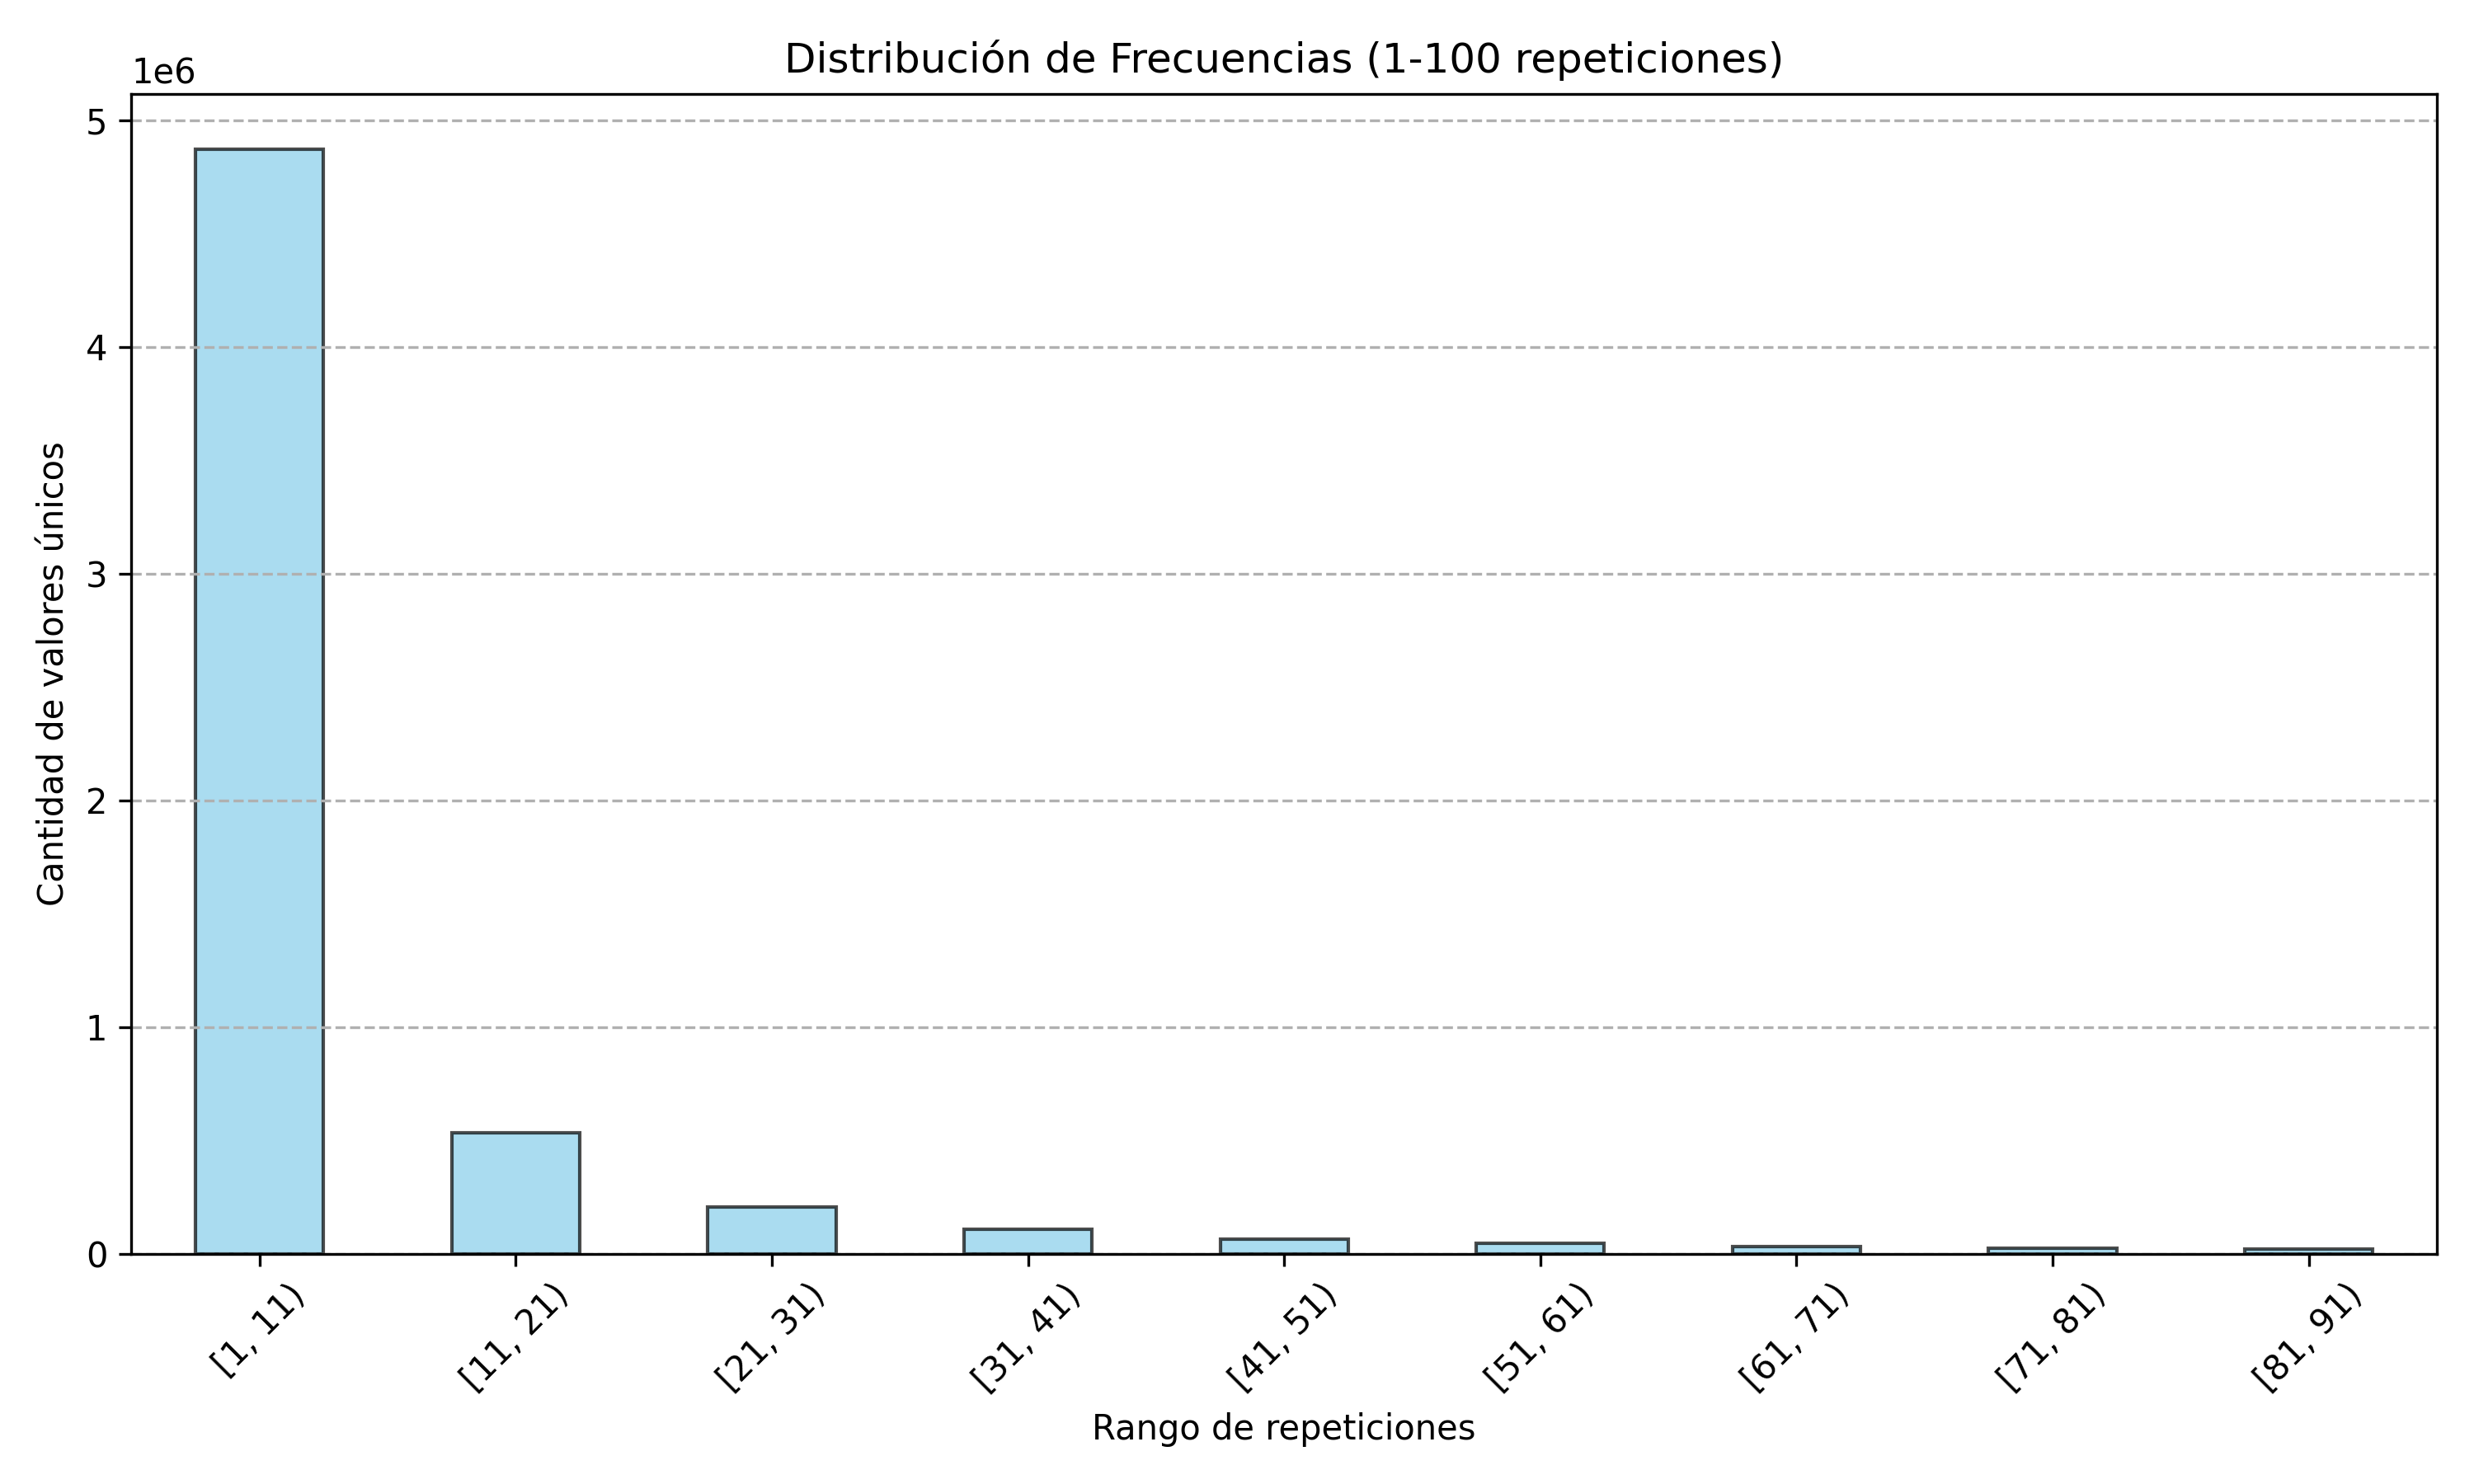
\includegraphics[width=\linewidth]{img/histograma_1_100.png}
        \caption{Histograma 1–100 repeticiones}
        \label{fig:sub1}
    \end{subfigure}
    \hfill
    \begin{subfigure}[t]{0.48\textwidth-1em}
        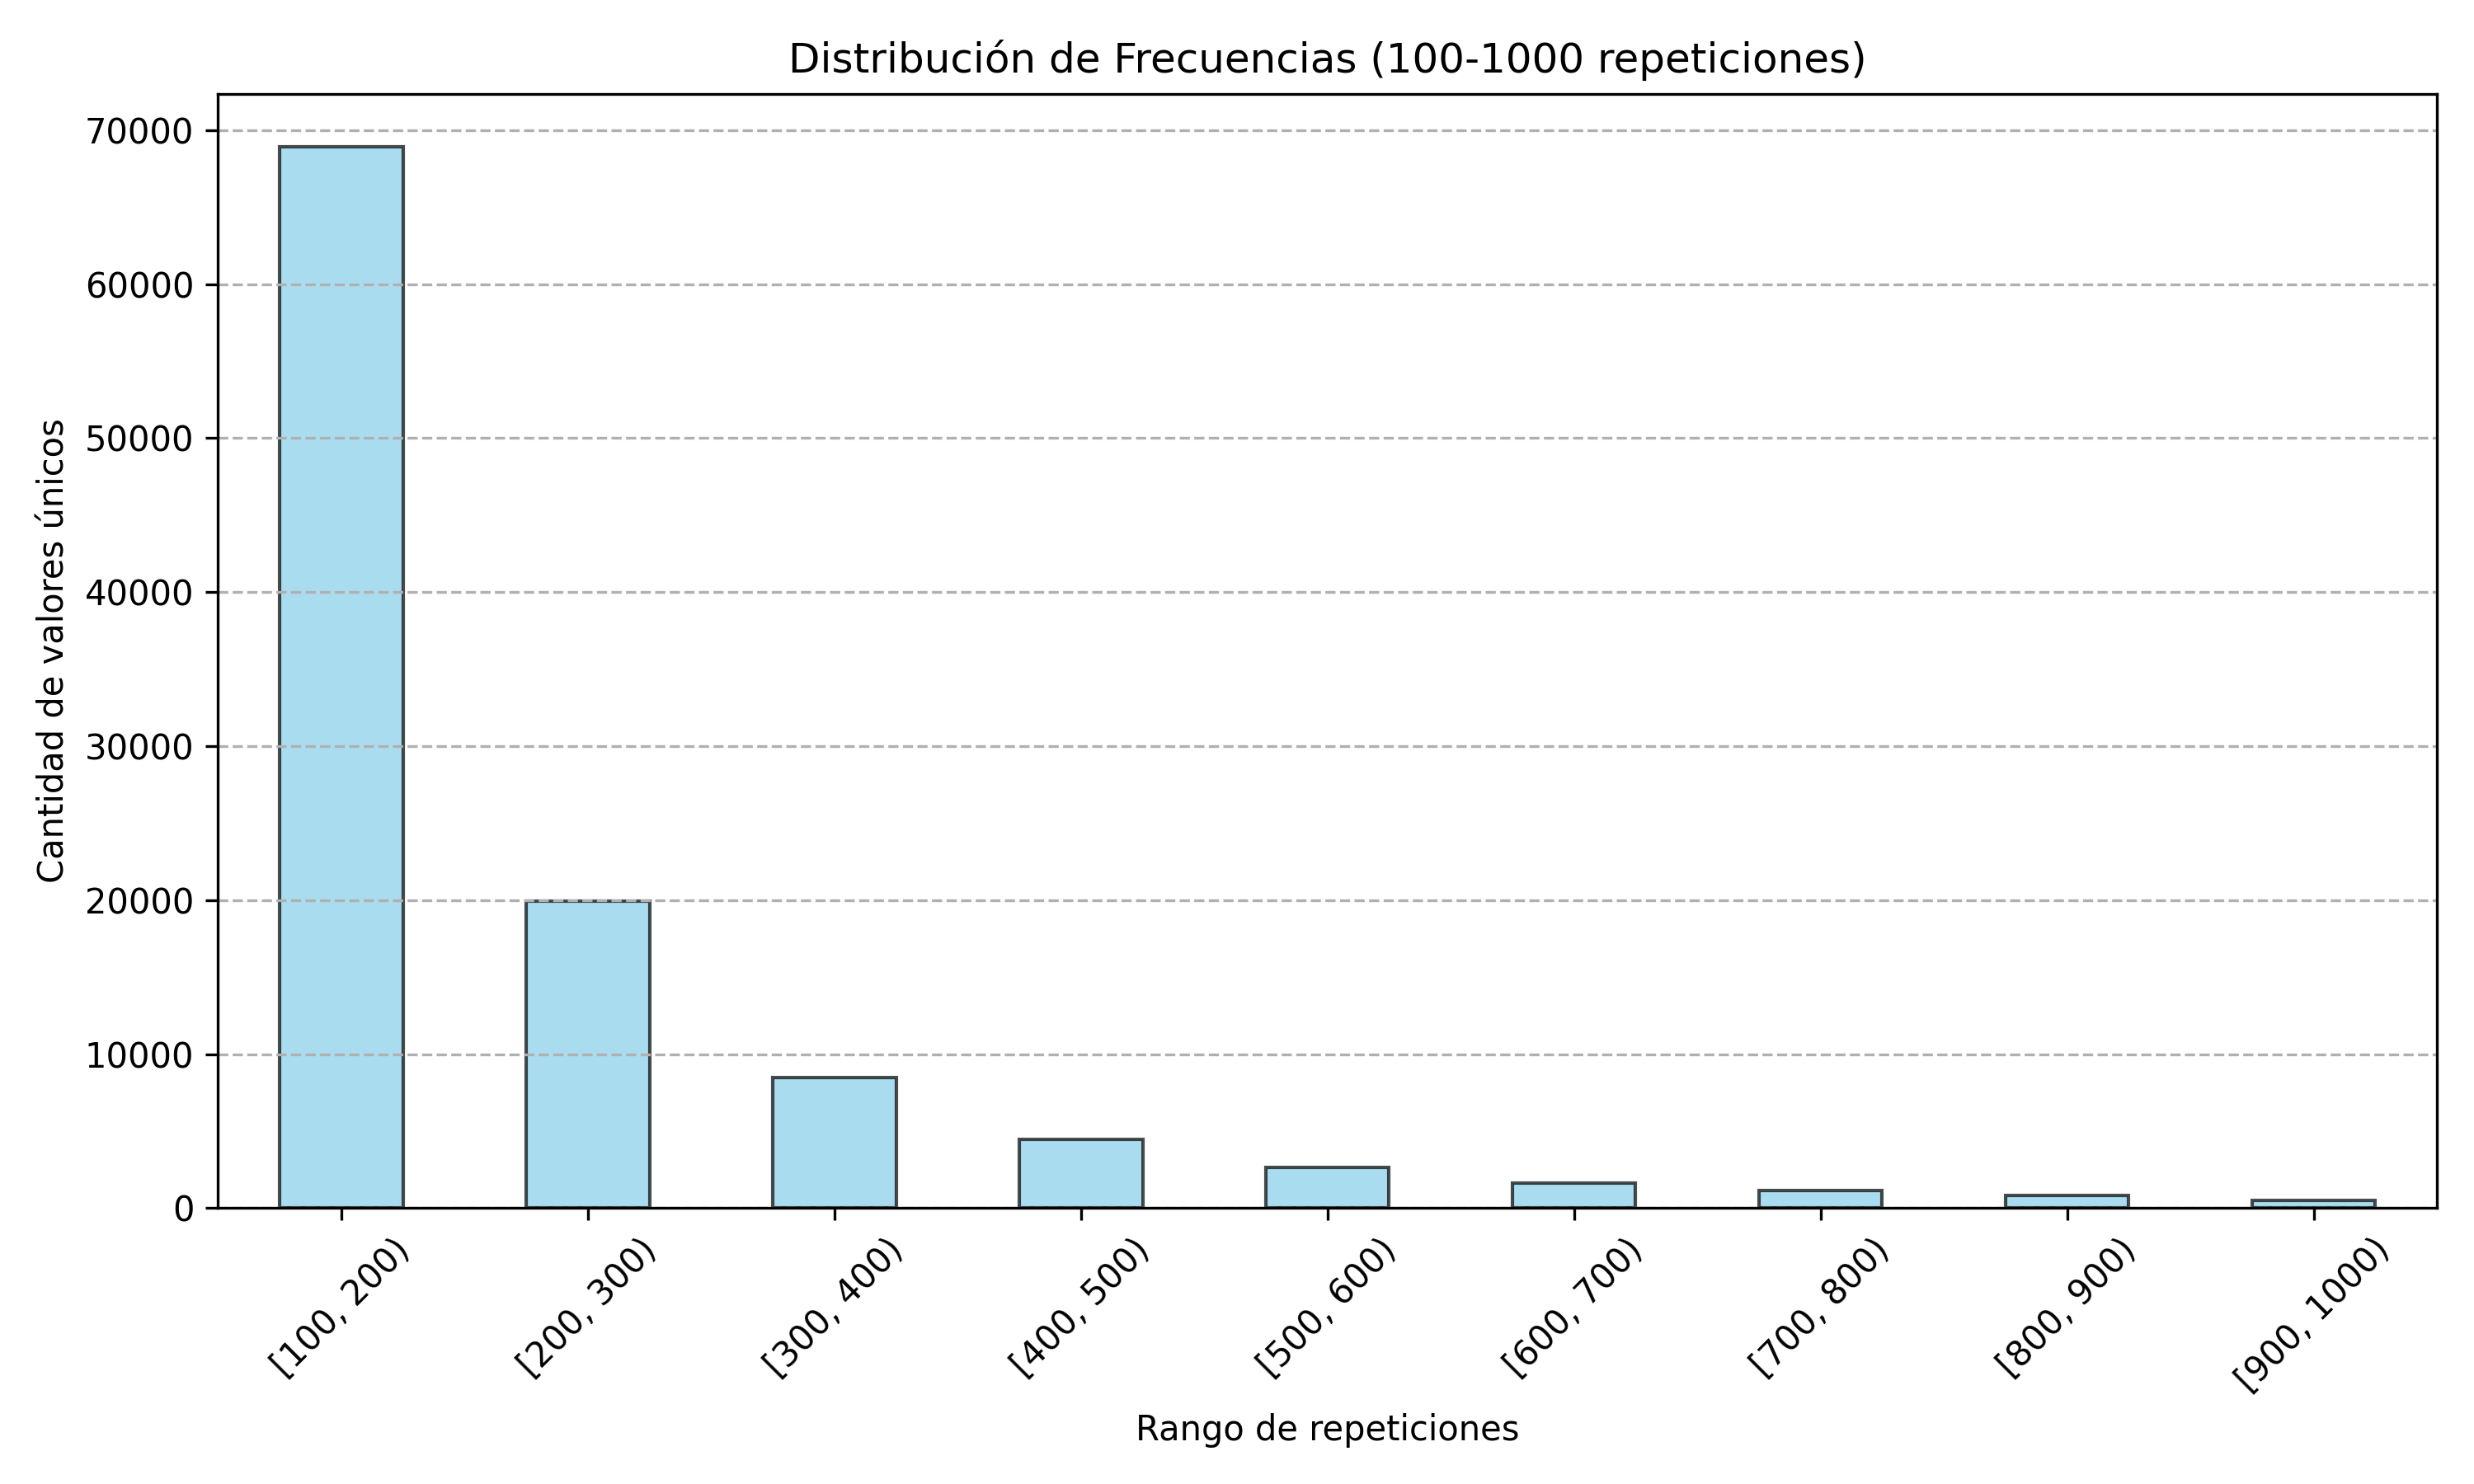
\includegraphics[width=\linewidth]{img/histograma_100_1000.png}
        \caption{Histograma 100–1000 repeticiones}
        \label{fig:sub2}
    \end{subfigure}

    \vspace{0.5cm}

    \begin{subfigure}[t]{0.48\textwidth}
        \centering
        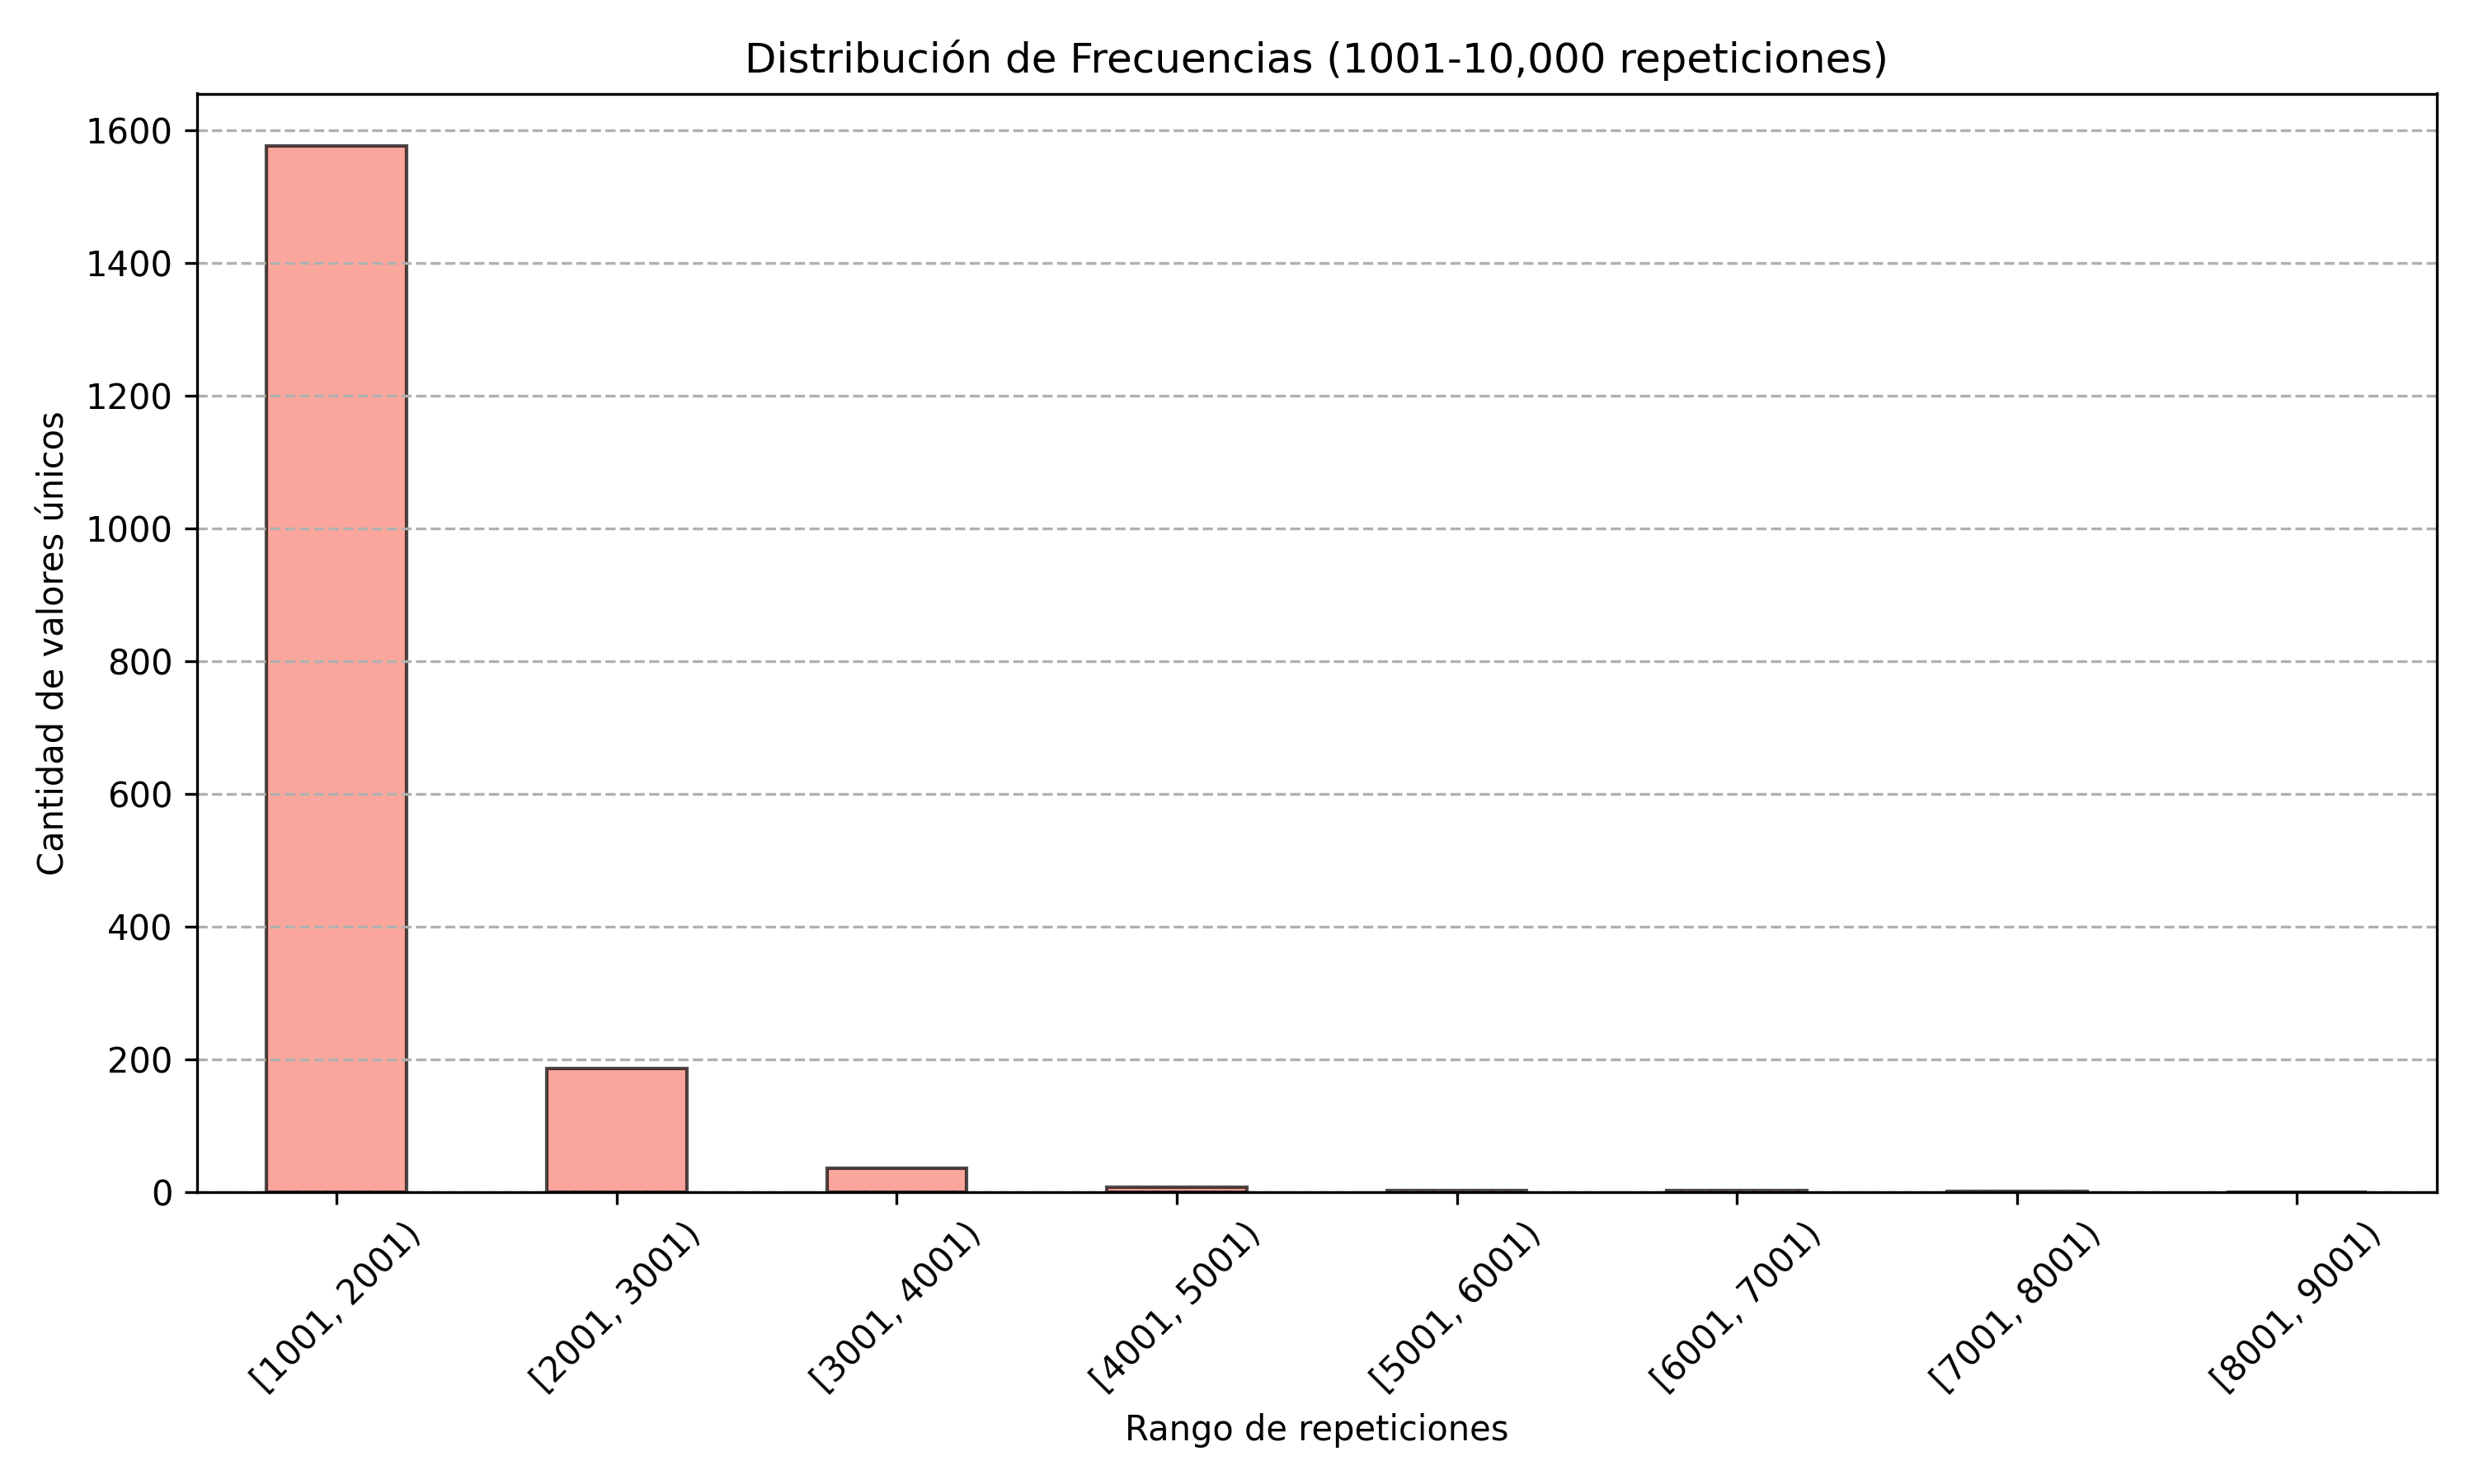
\includegraphics[width=\linewidth]{img/histograma_1001_10000.png}
        \caption{Histograma 1001–10000 repeticiones}
        \label{fig:sub3}
    \end{subfigure}

    \caption{Comparación de histogramas por rangos de repeticiones.}
    \label{fig:histogramas}
\end{figure}

Además de los histogramas, el script genera un resumen con el número total de valores únicos por rango:

\begin{verbatim}
        === Resumen de frecuencias ===
        **Rango 1 - 100 repeticiones**:
        - Total de valores únicos: 5,912,437

        **Rango 100 - 1000 repeticiones**:
        - Total de valores únicos: 108,519

        **Rango 1000 - 10000 repeticiones**:
        - Total de valores únicos: 1,816
\end{verbatim}

Esta información evidencia que la mayoría de los identificadores aparecen entre 1 y 100 veces, siendo predominante el subconjunto de 1 a 10 repeticiones. 

\newpage
Con base en esta información es necesario hacer un análisis más detallado de los identificadores. Para ello, se eliminan los registros que tienen duplicados, es decir, aquellos que tienen la misma información en las columnas \texttt{timestamp}, \texttt{device\_lat}, \texttt{device\_lon}. Después de aplicar este filtro se obtiene un total de \textbf{50,753,197}. 

\begin{figure}[H]
    \centering
    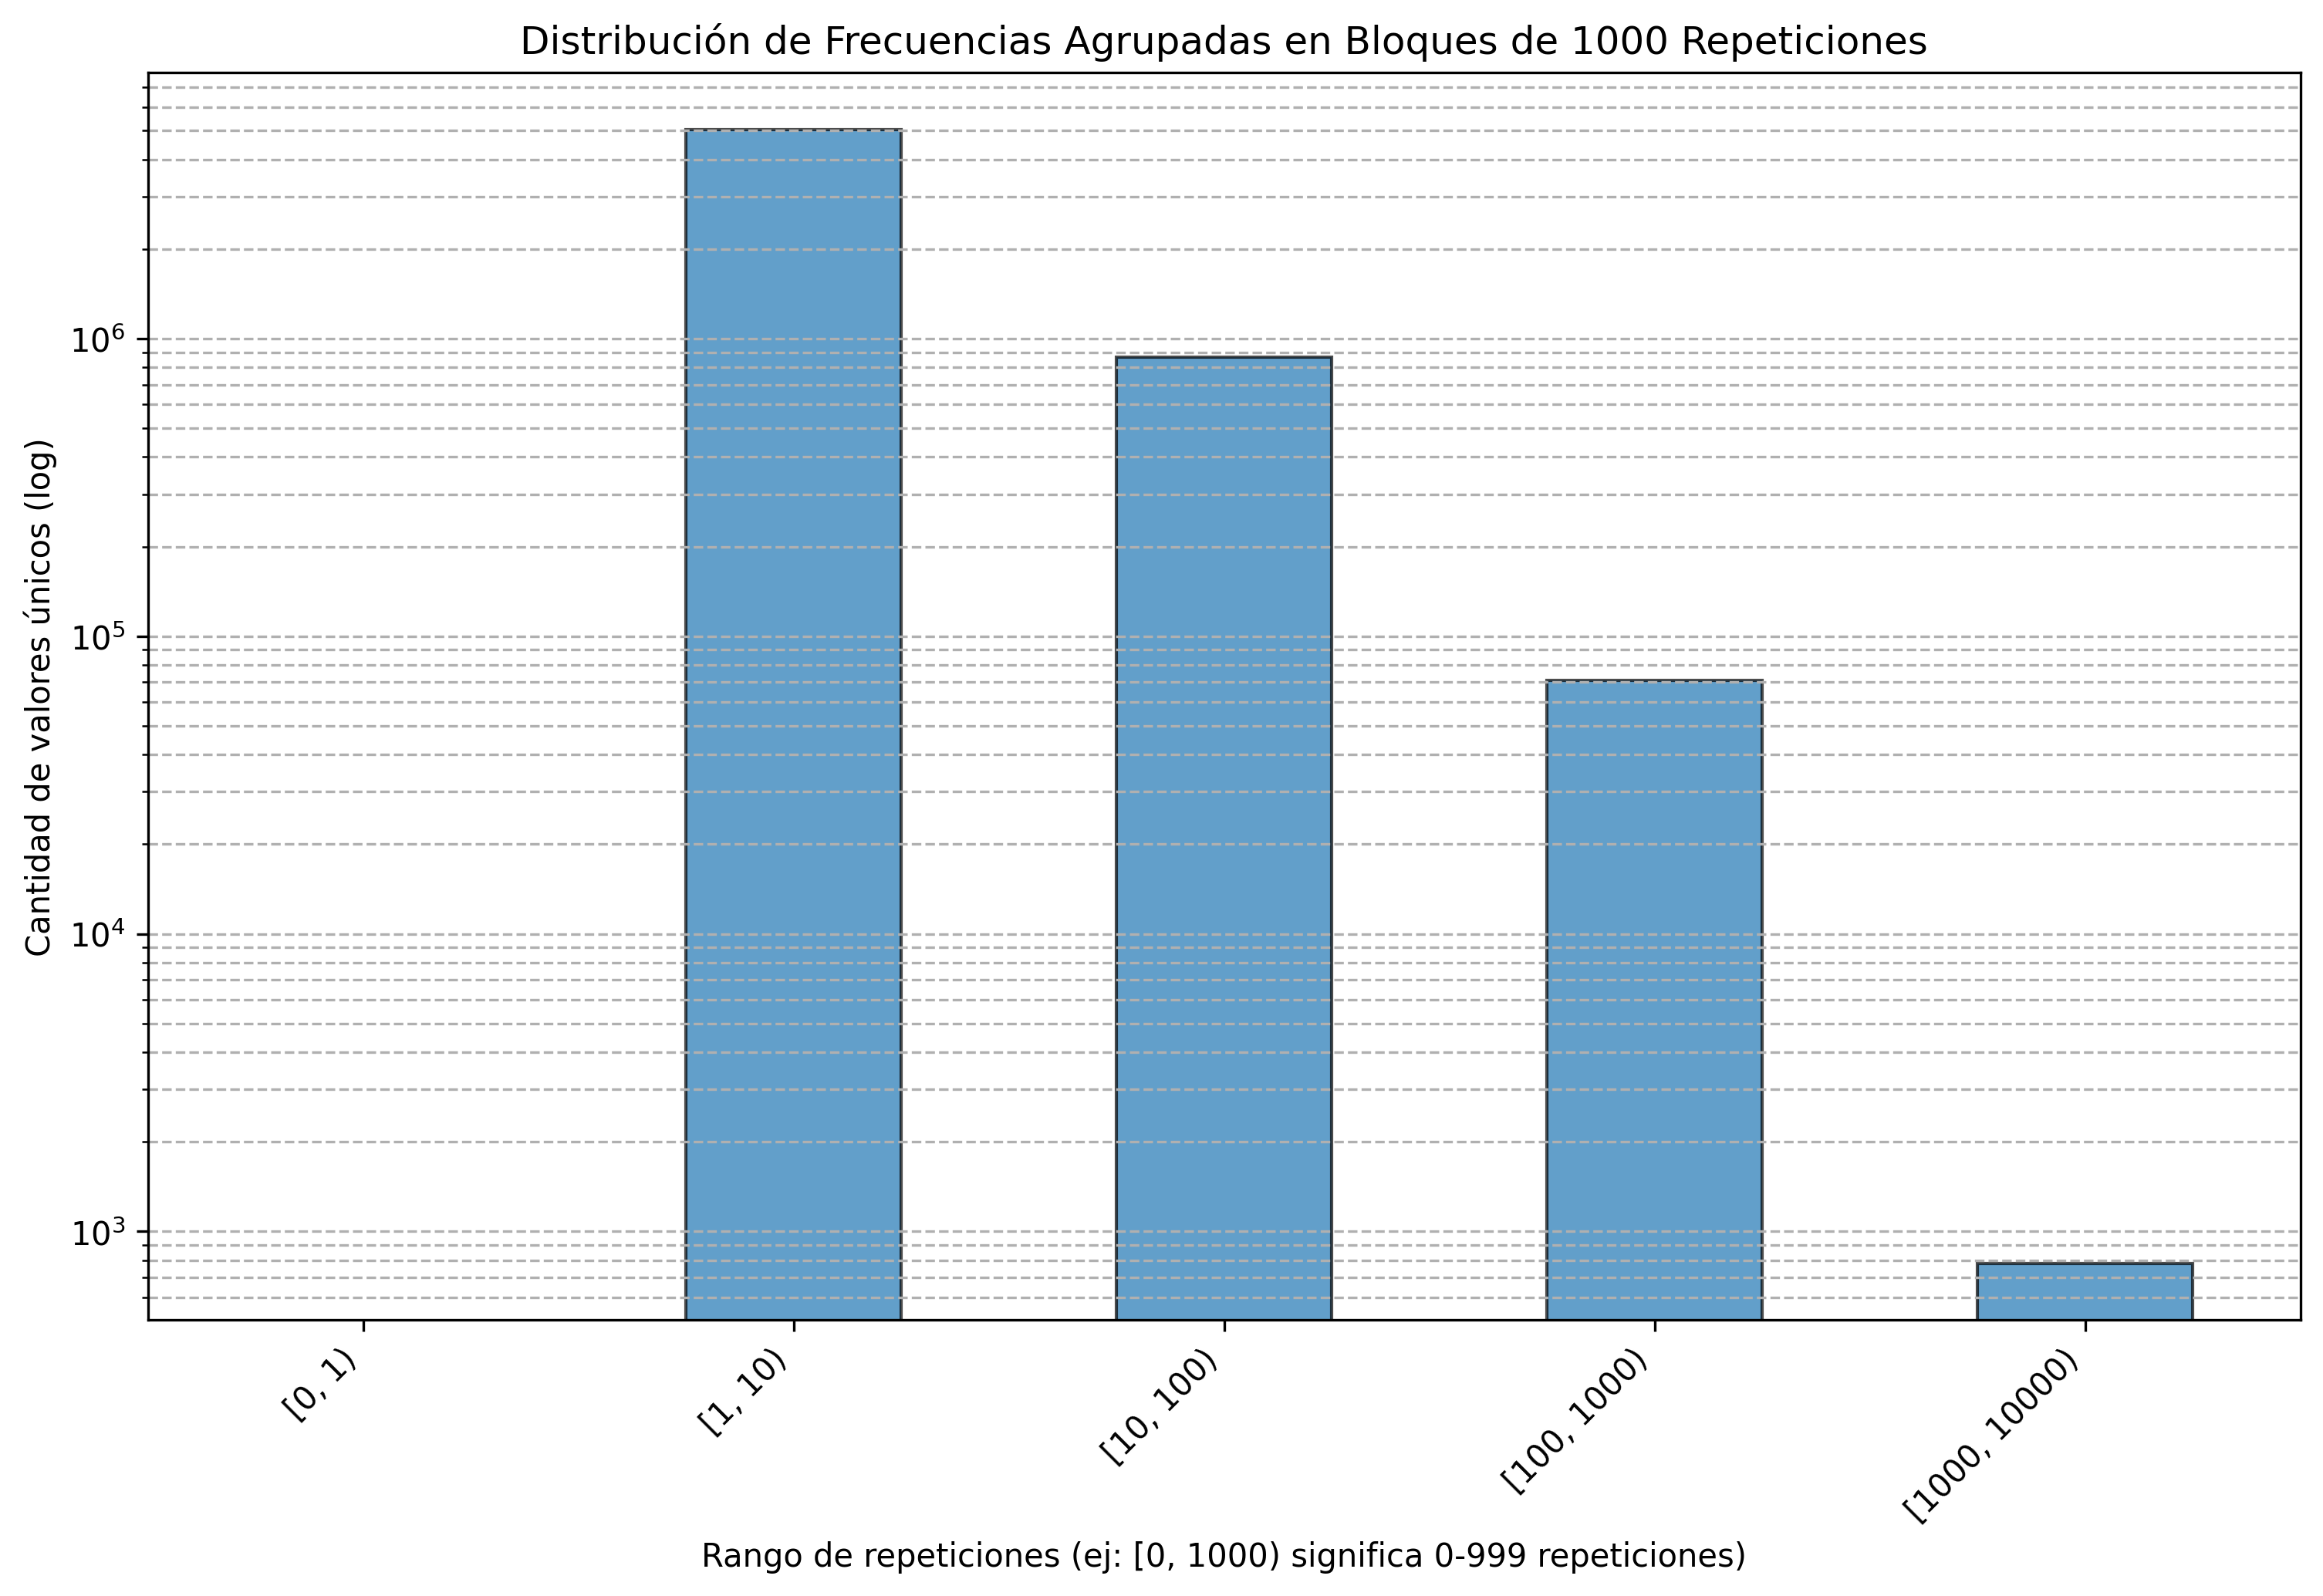
\includegraphics[width=\textwidth]{img/histograma_frecuencias_agrupadas_1000_dup.png}
    \caption{Frecuencias de valores agrupados por rangos (0–200 metros).}
    \label{fig:accuracy_histogram}
\end{figure}

